\documentclass[11pt, a4paper]{article}
\usepackage[utf8]{inputenc} % encoding multi-byte
\usepackage[top=2.5cm, bottom=2.5cm, left=2.5cm, right=2.5cm]{geometry}
\usepackage{amsmath,amssymb,amsfonts,latexsym,textcomp} %paquetes matematicos
\usepackage{array,multirow,booktabs,tabulary} %tablas y arrays
\usepackage{graphicx}   
\usepackage{caption,float,subfigure} %float=figuras flotantes.
\usepackage{verbatim}  %texto raw 
\usepackage[ampersand]{easylist} %http://en.wikibooks.org/wiki/LaTeX/List_Structures#Easylist_package 
\usepackage{subfigure}
\usepackage{color}
\usepackage[usenames,dvipsnames,svgnames,table,x11names]{xcolor} 
%\usepackage{parskip}
%\setlength{\parindent}{0pt}	


%---- Bibliografia bibtex+biblatex -----------------------------------------
\usepackage[backend=bibtex,backref,natbib,sorting=none]{biblatex} %backref=hyperlinks de inversa, e.g.(vid. pag. xx)	
\bibliography{week4.bib} 

\usepackage{fancyhdr}
\pagestyle{fancy}
\fancyhf{}
\lhead{Registration Number: 180123717}
\cfoot{\thepage}
%---- tikz ----------------------------------------------------------------
\usepackage{tikz}
\usetikzlibrary{calc,patterns,angles,quotes,decorations.pathmorphing,decorations.markings,circuits,arrows,positioning,shapes}

%---- subsubequations numbering  -----------------------------------
%https://tex.stackexchange.com/questions/58489/nested-subequations-following-equations-get-wrong-numbers
\makeatletter
\newcounter{parentsubequation}% Counter for ``parent equation''.
\newenvironment{subsubequations}{%
	\refstepcounter{equation}%
	\protected@edef\theparentsubequation{\theequation}%
	\setcounter{parentsubequation}{\value{equation}}%
	\setcounter{equation}{0}%
	\def\theequation{\theparentsubequation\alph{equation}}%
	\ignorespaces
}{%
	\setcounter{equation}{\value{parentsubequation}}%
	\ignorespacesafterend
}
\makeatother


%---- Hyperlinks  ----------------------------------------------------------
\usepackage[ %
breaklinks, %
colorlinks=true, %
linkcolor=black, %
citecolor=black, %
urlcolor=black %
]{hyperref} 

%---- Usar otros fonts + símbolo \degree -----------------------------------
\newcommand*{\myfont}{\fontfamily{lmtt}\selectfont}
\DeclareTextFontCommand{\textmyfont}{\myfont}	
\usepackage{gensymb} 

%---- Code highlighting con Listings ---------------------------------------
\usepackage{listings}	
\definecolor{mygreen}{rgb}{0.5,0.6,0.5}
\definecolor{mygray}{rgb}{0.5,0.5,0.5}
\definecolor{mymauve}{rgb}{0.58,0,0.82}
\definecolor{mygray2}{rgb}{0.9764, 0.9764, 0.9762}
%---- Config listings ------------------------------------------------------
\lstset{ %
	backgroundcolor=\color{mygray2},	% background color \color{mygray2}
	basicstyle=\footnotesize\ttfamily,	% tamaño de las letras y tipo de letra
	breaklines=true,	% corte de linea (line breaking)solo en espacio blanco
	captionpos=b,		% posicion del caption b,t,n (top,bottom,none)
	commentstyle=\color{ForestGreen},	% estilo del comentario
	%escapeinside={\%*}{*},	% si se desea agregar codigo Latex dentro el codigo debe ser %*codigo latex*
	frame=none,	% agrega marco al codigo (single)
	frameround=tttt,	% redondear el marco
	keepspaces=true,	% mantiene los espacios en el texto, util para mantener la indentacion del codigo (uso posible en columns=flexible)
	keywordstyle=\color{blue},	% estilo de los keywords
	stringstyle=\color{mymauve},	% estilo del string
	numbers=none,	% donde poner los numeros de linea, (none, left, right)
	numbersep=5pt,	% cuan lejos los numeros de linea estan del codigo
	xleftmargin=0pt,	% margen izquierdo
	showspaces=false,	% muestra espacios de codigo en todas partes usando el caracter barra baja "_", sobreescribe el comando 'showstringspaces'
	showstringspaces=false,	% muestra espacios solo en los strings
	tabsize=2,	% tabulacion por defecto =2
	title=\lstname	% muestra el nombre de lo archivos incluidos con \lstinputlisting; tambien se puede tratar con caption en vez de title
}	
%---- Config personalizada del caption -------------------------------------
\DeclareCaptionFont{white}{\color{black}}
\DeclareCaptionFormat{listing}{
%	\colorbox[cmyk]{0.43, 0.35, 0.35, 0.01 }{
%		\parbox{0.96\linewidth}{\hspace{15pt}#1#2#3}
%	}
	\colorbox{white}{
		\parbox{0.96\linewidth}{\centering #1#2#3}
	}
}
\captionsetup[lstlisting]{ format=listing, 
	labelfont=white, 
	textfont=white, 
	singlelinecheck=false, 
	margin=0pt, 
	font={bf,footnotesize} }
%---- Caracteres especiales ------------------------------------------------	
% Por defecto, listings no soporta inputec para mostrar los acentos y caracteres especiales.
% para manejar utf8 se debe enlistar los caracteres segun:
\lstset{literate=
	{á}{{\'a}}1 {é}{{\'e}}1 {í}{{\'i}}1 {ó}{{\'o}}1 {ú}{{\'u}}1
	{Á}{{\'A}}1 {É}{{\'E}}1 {Í}{{\'I}}1 {Ó}{{\'O}}1 {Ú}{{\'U}}1
	{à}{{\`a}}1 {è}{{\`e}}1 {ì}{{\`i}}1 {ò}{{\`o}}1 {ù}{{\`u}}1
	{À}{{\`A}}1 {È}{{\'E}}1 {Ì}{{\`I}}1 {Ò}{{\`O}}1 {Ù}{{\`U}}1
	{ä}{{\"a}}1 {ë}{{\"e}}1 {ï}{{\"i}}1 {ö}{{\"o}}1 {ü}{{\"u}}1
	{Ä}{{\"A}}1 {Ë}{{\"E}}1 {Ï}{{\"I}}1 {Ö}{{\"O}}1 {Ü}{{\"U}}1
	{â}{{\^a}}1 {ê}{{\^e}}1 {î}{{\^i}}1 {ô}{{\^o}}1 {û}{{\^u}}1
	{Â}{{\^A}}1 {Ê}{{\^E}}1 {Î}{{\^I}}1 {Ô}{{\^O}}1 {Û}{{\^U}}1
	{œ}{{\oe}}1 {Œ}{{\OE}}1 {æ}{{\ae}}1 {Æ}{{\AE}}1 {ß}{{\ss}}1
	{ç}{{\c c}}1 {Ç}{{\c C}}1 {ø}{{\o}}1 {å}{{\r a}}1 {Å}{{\r A}}1
	{ñ}{{\~n}}1 {£}{{\pounds}}1 {°}{{\degree}}1
}		
%---- Macro de inclusión de documentos con listings ------------------------
% [2]=numero de argumentos, #1=argumento 1, #2=argumento 2
\newcommand{\includecode}[2]{\lstinputlisting[language=#1, caption=#2, label=#2]{#2}}			
\renewcommand{\lstlistingname}{Code}
%=============================================================================================
%opening
\title{The University of Sheffield\\
	ACS6101 Foundations of Control Systems\\ 
	Week 4 Assignment}
\author{Paulo Roberto Loma Marconi\\ \url{prlomarconi1@sheffield.ac.uk}}
\date{November 4, 2018}

\begin{document}
\maketitle

\section{Question 1}
The aim of this task is to design a Phase-lead compensator using the Bode analysis in the frequency domain, and evaluate it in Matlab. Although the plant $G(s)$ is a third-order system Eq.\eqref{eq:G}, the design requirements can be approximated in terms of the natural frequency ($\omega_n$) and damping ratio ($\zeta$) of a second-order system.

\begin{align}
& G(s)=\dfrac{K}{s(s+a)(s+b)} \label{eq:G}\\
& G(s)=\dfrac{K}{s(s+2.5)(s+27)} \nonumber
\end{align} 

\subsection{Determine the gain $K$ for a step response overshoot no more than 10\%}
There are two steps to follow in order to obtain the required gain $K$, the first one uses the second-order performance approximation in the frequency domain, and the second step uses the gain and angle condition.

The relation between the Percentage Overshoot ($P.O.$) in response to a unity step input of a second-order system in the \textbf{time domain}, and the Phase Margin ($PM$) of the Bode analysis in the \textbf{frequency domain}, can be written as follows,
\begin{align}
& P.O. = 100~e^{-\zeta\pi/\sqrt{1-\zeta^2}} \label{PO} \\
& PM  \approx 100 ~\zeta \label{eq:PM}
\end{align}
applying the requirement of $P.O.\leq10\%$,
\begin{align}
& \zeta = \dfrac{ \ln\left(\frac{100}{P.O.}\right) }{\sqrt{\pi^2+\left[ \ln \left(  \frac{100}{P.O.}\right)\right]}}	\label{eq:zeta} \\
& \zeta = 0.59 \approx 0.60 \nonumber
\end{align}
Using Eq.\eqref{eq:PM}, the desired Phase Margin ($PM_d$) the system should have in order to satisfy the $P.O.$ is defined as,
\begin{align*}
PM_d = 100\times 0.6 = 60\degree
\end{align*}

Now, it is necessary to obtain the new crossover frequency ($\omega_c^\prime$) where the $PM_d$ is satisfied. Using the $PM_d$ equation and the phase angle condition ($\phi(\omega_c^\prime)$)  as follows,
\begin{align}
&\phi(\omega_c^\prime) = -180\degree + PM_d\\
\intertext{applying the rule of angles into the Eq.\eqref{eq:G},}
&\phi(\omega_c^\prime) = -90\degree - \arctan \frac{\omega_c^\prime}{a} - \arctan \frac{\omega_c^\prime}{b}\\
\intertext{and after some algebraic operations $\omega_c^\prime$, }
& PM_d - 180\degree  = -90\degree - \arctan \frac{\omega_c^\prime}{a} - \arctan \frac{\omega_c^\prime}{b}   \nonumber\\
& \frac{\omega_c^\prime(a+b)}{a~b} = \left(1-\frac{\omega_c^{\prime 2}}{a~b}\right) \tan(180\degree - 90\degree -PM_d) \nonumber \\
\intertext{solving the quadratic equation with the corresponding values $a$, $b$, and $PM_d$, and using the high value of the solution,}
&  \omega_c^{\prime 2}  + \frac{a+b}{\tan(180\degree - 90\degree -PM_d)} \omega_c^\prime - a~b = 0\\
& \omega_c^\prime  = 1.29 ~rad/sec \nonumber
\end{align}

Finally, the gain $K$ can be obtained from the \textbf{gain condition}, where it is established that the new crossover frequency $\omega_c^\prime$ should be at $0~dB$ of magnitude, in other words,
\begin{align}
& \arrowvert G(j\omega_c^\prime) \arrowvert = 1 \label{eq:GainCondtion}\\
\intertext{applying into the plant $G$, Eq.\eqref{eq:G}, and replacing the values}
&\dfrac{K}{\omega_c^\prime \sqrt{\omega_c^{\prime 2}+a^2} \sqrt{\omega_c^{\prime 2}+b^2 }} = 1 \nonumber\\
& K	= \omega_c^\prime \sqrt{\omega_c^{\prime 2}+a^2} \sqrt{\omega_c^{\prime 2}+b^2 } \nonumber\\
& K = 97.96 \nonumber
\intertext{therefore, the plant becomes,}
& G(s)=\dfrac{97.96}{s(s+2.5)(s+27)} \nonumber
\end{align}

In Fig. \ref{fig:Q1_a}a it can be seen that the desired $PM_d = 60\degree$ is satisfied with the new gain, and step response has an $P.O. = 8.36$.

\begin{figure}[H]
	\centering
	\subfigure[Bode plot]{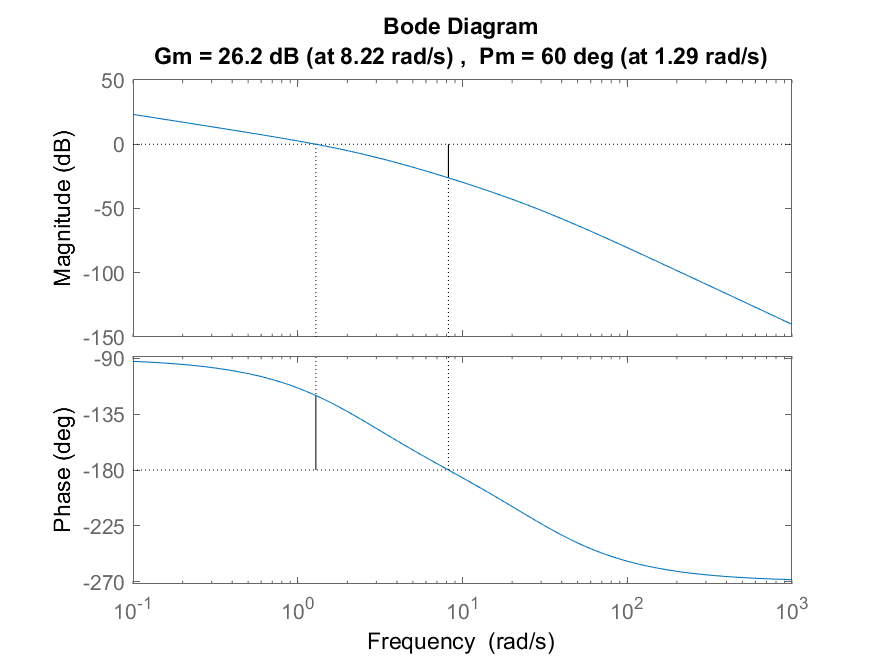
\includegraphics[width=0.44\linewidth]{../Q1_a_margin.png}}
	\subfigure[Step response]{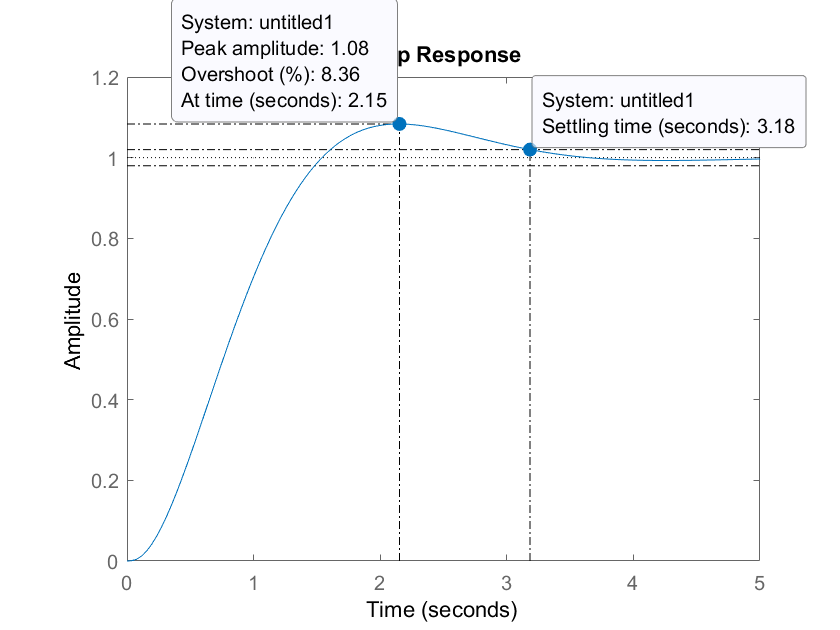
\includegraphics[width=0.44\linewidth]{../Q1_a_step.png}}
	\caption{Evaluation of the system with the new gain }
	\label{fig:Q1_a}
\end{figure}

The following script in Matlab simulates the previous results.

\begin{lstlisting}[language=matlab, caption={}, label={}]
%% ========================================================================
% ---- ACS6101 Assignment week 4
% ---- Registration number: 180123717
% ---- Name: Paulo Roberto Loma Marconi
% ---- 23/10/2018
%% === Question 1 =========================================================
clear; clc; close all;
%% plant G parameters
s = tf('s');
a = 2.5; b = 27;
%% a) Gain K for PO=10
PO = 10; % percentage overshoot
zeta = log(100/PO)/sqrt(pi^2+ (log(100/PO))^2 ); % damping ratio
PM_d = round(100*zeta)+1; % PM desired at the nearest round value
h = tand(180-90-PM_d); 
omega_c = roots([1 (a+b)/h -a*b]); % new omega_c
K = omega_c(2)*sqrt(omega_c(2)^2+a^2)*sqrt(omega_c(2)^2+b^2); % new gain K
G = K/( s*(s+a)*(s+b) ); % Plant G
fig = figure(1);
margin(G);
saveas(fig,'Q1_a_margin.png');
fig = figure(2);
step(feedback(G,1));
saveas(fig,'Q1_a_stepp.png');
\end{lstlisting}


\subsection{Design of the Phase-lead compensator}
The Phase-Lead compensator has the following transfer function,
\begin{align}
Gc = \dfrac{s+z}{s+p} \label{eq:Gc_lead}
\end{align}
where the location of the zero is to the left of the pole, $|z|<|p|$.

The design requirements are the velocity error constant $K_v\leq 25$, and the step response $P.O.\leq 10\%$

The first step is to calculate the loop gain that satisfies the $K_v$ is calculated as follows,
\begin{align}
K_v &= \lim\limits_{s \rightarrow 0} s \dfrac{K}{s(s+2.5) (s+27)} \\
K_g &= 1687 \nonumber\\
\intertext{therefore, the new plant is,} 
G(s) &= \dfrac{K_g}{s(s+a)(s+b)} \\
G(s) &= \dfrac{1687}{s(s+2.5)(s+27)} \nonumber
\end{align}

Using the Eq.\eqref{PO}, Eq.\eqref{eq:zeta}, Eq.\eqref{eq:PM}, it is obtained that for an overshoot of $P.O.=10 \%$, the damping ratio is $\zeta = 0.6$, and the desired phase margin is $PM_d=60\degree$.

In order to obtain the  $\omega_c$ that satisfies the gain condition with the new gain $K$, Eq.\eqref{eq:GainCondtion} is applied as follows,
\begin{align}
&\arrowvert G(j\omega_c) \arrowvert = 1 \nonumber\\
&\left| \dfrac{K_g}{j\omega_c(j\omega_c+a)(j\omega_c+b)} \right| = 1 \nonumber\\
\intertext{after some algebraic operation, }
&\omega_c^2(\omega_c^2+a^2)(\omega_c^2+b^2)-K_g^2 = 0 \nonumber \\
&\omega_c = 7.55 ~rad/sec \nonumber
\end{align}
Now, the actual phase margin $PM_{act}$ is needed to calculate the additional phase ($\phi_m$) required from the compensator,
\begin{align}
PM_act &= 180\degree + \phi(\omega_c) \\
PM_act &= 180\degree - 90\degree -\arctan \frac{\omega_c}{a} - \arctan \frac{\omega_c}{b} \nonumber \\
PM_act &= 2.65 \nonumber\\
\intertext{so, the additional phase angle is,} 
\phi_m &= PM_d+\theta-PM_act \\
\intertext{where $\theta$ is a factor of correction. If $\theta=0$,}
\phi_m &= 60\degree + 0\degree - 2.65 \nonumber\\
\phi_m &= 57 \degree \nonumber
\end{align}

The additional phase margin is related with the zero and the pole of the Phase-Lead compensator as follows,
\begin{align}
\alpha &= \dfrac{\sin \phi_m+1}{1-\sin \phi_m} \\
\alpha &= 11 \nonumber \\
\intertext{where $\alpha$ is,}
\alpha &= \dfrac{p}{z}  \label{eq:alpha}
\end{align}
The next step is to determine the new $\omega_c^\prime$ using the following logarithm gain condition,
\begin{align}
&20\log|G(j\omega_c^\prime)| = -10 \log \alpha\\
&\dfrac{K_g}{\omega_c^\prime \sqrt{\omega_c^{\prime 2}+a^2} \sqrt{\omega_c^{\prime 2}+b^2 }} = \dfrac{1}{\sqrt{\alpha}}\\
\intertext{after some operations,}
&\omega_c^{\prime 2}(\omega_c^{\prime 2}+a^2)(\omega_c^{\prime 2}+b^2)-K_g^2~\alpha = 0 \nonumber \\
&\omega_c^\prime = 13.50 ~rad/sec \nonumber
\intertext{now, calculating the zero of the compensator,}
\omega_c^\prime &= \sqrt{p~z} \\
z &= \dfrac{\omega_c^\prime}{\alpha} \nonumber\\
z &= 4.07 \nonumber\\
\intertext{and the pole of the compensator using Eq.\eqref{eq:alpha} is,}
p &= \alpha ~z \nonumber\\
p &= 44.78 \nonumber
\intertext{The last step is to obtain the new gain of the \textbf{compensated system,}}
K_{new} &= \sqrt{\alpha} K_g \\
K_{new} &= 5596.80 \nonumber\\
\intertext{therefore, the compensated open-loop transfer function is as follows,}
G_{ol} &= \dfrac{s+z}{s+p} \quad \dfrac{K_{new}}{s(s+a)(s+b)} \\
G_{ol} &= \dfrac{s+4.07}{s+44.78} \quad \dfrac{5596.80}{s(s+2.5)(s+27)} \nonumber
\end{align}

The following Matlab script calculates the Phase-Lead compensator with the design requirements.
\begin{lstlisting}[language=matlab, caption={}, label={}]
%% b) Phase-lead compensator
Kv = 25; % velocity error
Kg = Kv*a*b; % loop gain to satisfy Kv
G = Kg/( s*(s+a)*(s+b) ); % Plant G
% omega_c for the uncompensated system
omega_c = real( sqrt( roots([1 a^2+b^2 a^2*b^2 -Kg^2]) ) );
% obtaining actual PM
PM_act = 180-90-atand(omega_c(3)/a)-atand(omega_c(3)/b);
% additional phase angle from the compensator PM
theta = 0; % factor of correction
PM_c = round(PM_d+theta-PM_act);
% calculating alpha
alpha = round( (sind(PM_c)+1)/(1-sind(PM_c)) );
% Determine the new cross over frequency
omega_c_new = real( sqrt( roots([1 a^2+b^2 a^2*b^2 -Kg^2*alpha]) ) );
% Calculating the zero of the compensator
z = omega_c_new(3)/sqrt(alpha);
% Calculating the pole of the compensator
p = alpha*z;
% lead compensator
Gc = (s+z)/(s+p);
% new gain of the compensated system
K_new = sqrt(alpha)*Kg;
% compensated open-loop 
Gol = K_new*Gc*G/Kg;
% closed-loop 
Gcl = feedback(Gol,1);
\end{lstlisting}

\subsection{Evaluation of the compensated system to a unit ramp input}
The unit ramp in the LaPlace domain has the following equation,
\begin{align}
R(s) &= \frac{1}{s^2}\\
\intertext{and the steady-state error to that unit ramp is,}
ess_v &= \frac{1}{K_v} \\
\intertext{where,}
K_v &= \lim\limits_{s\rightarrow 0} s~G(s) \\
\intertext{evaluating $K_v$ for the compensated system $G_{ol}$,}
K_v &= \lim\limits_{s\rightarrow 0} s~ \left[\dfrac{s+z}{s+p} \quad \dfrac{K_{new}}{s(s+a)(s+b)} \right] \nonumber\\
K_v &= 7.53 \nonumber
\intertext{therefore,}
ess_v &= 0.13 \nonumber\\
\intertext{which is a relatively small steady-state error. }
\end{align}


\subsection{Evaluation the performance of the compensated system}
Fig. \ref{fig:Q1_lead} shows the Bode plot, unit step response, and the unit ramp response. It can be seen that the desired $PM_d=60\degree$ and the $P.O.=10\%$ is satisfied, and the system has an improved the settling time, $t_s=1.04$, see Table \ref{tab:lead}.


\begin{figure}[H]
	\centering
	\subfigure[Bode plot.]{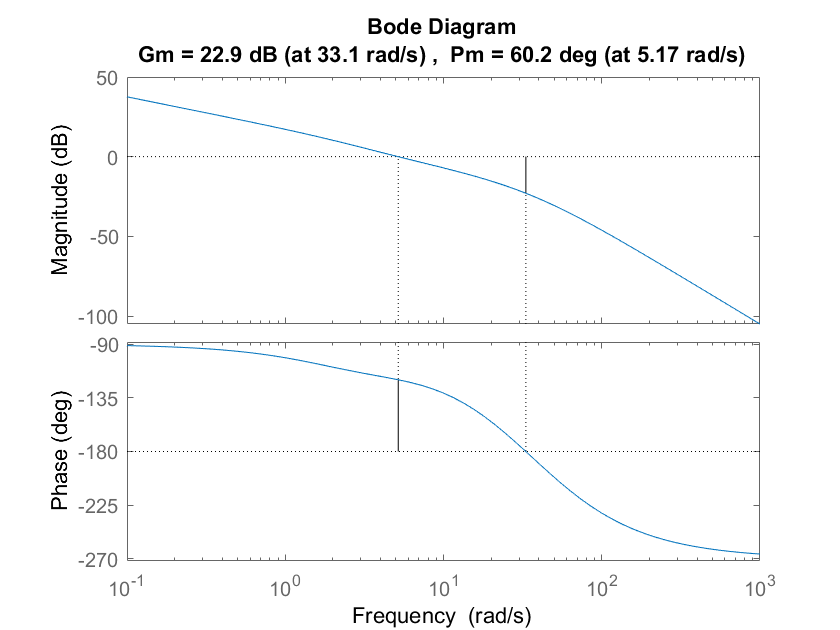
\includegraphics[width=0.48\linewidth]{../Q1_d_margin_lead.png}}
	\subfigure[Step and ramp response.]{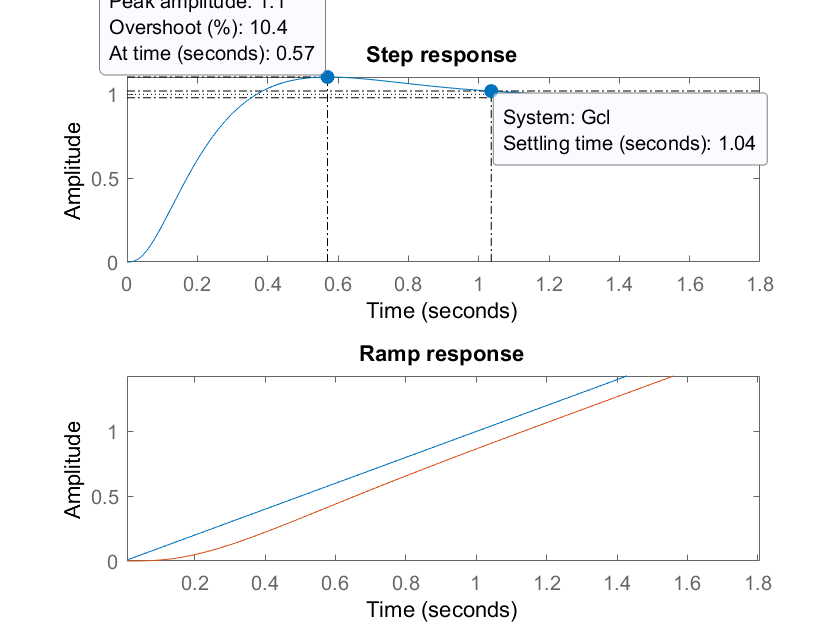
\includegraphics[width=0.48\linewidth]{../Q1_d_step_ramp_lead.png}}
	\caption{Evaluation of the compensated system.}
	\label{fig:Q1_lead}
\end{figure}

\begin{table}[!ht]
	\centering
	\scalebox{1}{
		\begin{tabular}{l|c}
			\bf{Quantity}                     & \bf{Value}  \\ \hline
			Steady state error to a unit ramp &    0.13      \\ \hline
			Rise Time                         &    0.24      \\ \hline
			Settling Time                     &    1.04      \\ \hline
			Percentage Overshoot              &   10.38      \\ \hline
			Phase Margin                      &   60.20      \\ \hline
			Gain Margin                       &   22.90      \\ \hline
			Bandwidth                         &    8.19      \\ \hline
			Peak Magnitude                    &    0.57      \\ \hline
			Resonant frequency                &    3.42      \\ \hline
		\end{tabular} 		
	}
	\caption{Performance evaluation. }
	\label{tab:lead}
\end{table}

The following Matlab script was used to obtain Fig. \ref{fig:Q1_lead}.

\begin{lstlisting}[language=matlab, caption={}, label={}]
%% c) evaluating the system to unit step and unit ramp
figure(2);
margin(Gol);
figure(3);
subplot(2,1,1);
step = 1/s; % step input
impulse(step,Gcl*step); 
title('Step response');
subplot(2,1,2);
ramp = 1/s^2; % ramp input
impulse(ramp,Gcl*ramp);
title('Ramp response');
% evaluating Kv for the new compensated system
Kv_new = (z/p)*K_new/(a*b);
% steady-state error to a unity ramp
ess_ramp = 1/Kv_new;
stepinfo(Gcl)
% bandwidth of Gcl
BW = bandwidth(Gcl);
% resonant frequency
omega_r = 4/(0.6*1.03) *sqrt(1-2*0.6^2);
\end{lstlisting}


\subsection{Conclusion}
Comparing the uncompensated system in Fig. \ref{fig:Q1_a}, and the Phase-Lead compensated system in Fig. \ref{fig:Q1_lead}, the desired phase margin $PM_d=60\degree$ and the overshoot $P.O.\leq10 \%$ were satisfied. Moreover, the settling time $t_s$ was improved three times in the Phase-lead compensated, which demonstrates this compensator improves the transient response without altering the desired phase margin.

\section{Question 2}
The objective of this task is to design a Phase-Lead compensator, and a Phase-Lag compensator in series with a the first Phase-Lead compensator using two different approaches. 

The plant to be studied is,
\begin{align}
& G(s)=\dfrac{K}{s^2(s+a)(s+b)} \label{eq:G2}\\
& G(s)=\dfrac{K}{s^2(s+9)(s+50)} \nonumber
\end{align} 

\subsection{Determine the location of closed-loop dominant poles}
The design requirements are the settling time $t_s\leq 2.9~ sec$, and the overshoot $P.O.\leq 20\%$. Although the plant is a fourth-order system, the compensator can be designed using the properties of a second-order system. 

The settling time is,
\begin{align}
t_s &= \frac{4}{\zeta\omega_n} \label{eq:ts}\\
\intertext{where $\zeta$ is the damping ration and $\omega_n$ is the natural frequency. Using Eq.\eqref{eq:zeta}, and Eq.\eqref{eq:ts},}
\zeta &= 0.45, \quad \omega_n = 3.06 ~rad/sec \nonumber\\
\intertext{therefore, the desired closed-loop dominant poles are,}
r_{1,2} &= -\omega_n\zeta\pm j~\omega_n\sqrt{1-\zeta^2}\\
r_{1,2} &= -1.38\pm j~2.73 \nonumber
\end{align}

The following Matlab script calculates the previous results.
\begin{lstlisting}[language=matlab, caption={}, label={}]
%% ========================================================================
% ---- ACS6101 Assignment week 4
% ---- Registration number: 180123717
% ---- Name: Paulo Roberto Loma Marconi
% ---- 27/10/2018
%% === Question 2 =========================================================
clear; clc; close all;
%% plant G parameters
s = tf('s');
a = 9; b = 50;
%% a) Location of the dominant poles for PO=20 and ts=2.9
PO = 20; % percentage overshoot
ts = 2.9; % settling time
zeta = log(100/PO)/sqrt(pi^2+ (log(100/PO))^2 ); % damping ratio
zeta = round(zeta,2)-0.01;
omega_n = 4/(zeta*ts);
% desired location of dominant poles
s1 = -omega_n*zeta+omega_n*sqrt(1-zeta^2)*1i;
\end{lstlisting}

\subsection{Demonstrate the desired poles do not belong to the root locus }
In order to demonstrate that the desired dominant poles $r_{1,2}$ do not belong to the root locus of the plant $G(s)$, the angle condition must not be satisfied,

Choosing on pole, $r_1=-1.38\pm j~2.73$, 
\begin{align}
&\measuredangle(G(r_1)) = -180\degree  \\
&\measuredangle \left( \dfrac{K}{r_1^2(r_1+9)(r_1+50)} \right) = 180\degree \nonumber\\
&-\measuredangle r_1 -\measuredangle r_1 - \measuredangle(r_1+9) - \measuredangle (r_1+50) = -80\degree \nonumber\\
&- 2~ \arctan \frac{2.73}{-1.38} - \arctan \frac{2.73}{9-1.38} - \arctan \frac{2.73}{50-1.38} = -180\degree \nonumber\\
&103.44 \neq -180\degree \nonumber
\intertext{if the second pole $r_2$ is evaluated,}
&-103.44 \neq -180\degree \nonumber
\end{align}



\subsection{Design of the Phase-Lead compensator}
The Phase-Lead compensator has the following transfer function,
\begin{align}
G_{lead} = \dfrac{s+z_{lead}}{s+p_{lead}}, \quad |z_{lead}| < |p_{lead}|
\end{align}
The design requirement is that the location of the compensator's zero is 1. Once again, the angle criteria is applied with the desired pole $r_1$ as follows,
\begin{align}
&\measuredangle \left( \dfrac{s+z_{lead}}{s+p_{lead}} \quad \dfrac{K}{s^2(s+a)(s+b)}  \right) = -180\degree \\
&\measuredangle \left( \dfrac{r_1+z_{lead}}{r_1+p_{lead}} \quad \dfrac{K}{r_1^2(r_1+a)(r_1+b)}  \right) = -180\degree \nonumber \\
&\measuredangle z_{lead} -\measuredangle p_{lead}- 2~\measuredangle s -\measuredangle a - \measuredangle b = -180\degree \nonumber\\
\intertext{if, $r_1 = -x+j~y$ }
&\left( 180\degree-\arctan\dfrac{y}{x-z_{lead}} \right) - \arctan\dfrac{y}{p_{lead}-x} - 2\left( 180\degree -\arctan\dfrac{y}{x} \right) ... \nonumber\\
&\quad -\arctan\dfrac{y}{a-x}-\arctan\dfrac{y}{b-x} = 180\degree \nonumber
\end{align}
after some operations,
\begin{align}
p_{lead} &= 8.36 \nonumber\\
\intertext{so, the Phase-Lead compensator is,}
G_{lead} &= \dfrac{s+1}{s+8.36} \nonumber
\end{align}

Now, the gain $K$ of the compensated system can be found using the gain condition,
\begin{align}
&\left|  \dfrac{s+z_{lead}}{s+p_{lead}} \quad \dfrac{K}{s^2(s+9)(s+50)} \right| = 1 \nonumber\\
&\left|  \dfrac{r_1+1}{r_1+8.38} \quad \dfrac{K}{r_1^2(r_1+9)(r_1+50)} \right| = 1 \nonumber\\
&K = 10047 \nonumber
\end{align}

Therefore, evaluating the following open-loop compensated system,
\begin{align}
G_{ol} &= G_{lead} ~G(s) \label{eq:Gol_lead}\\ 
G_{ol} &= \dfrac{s+1}{s+8.36}~ \dfrac{10047}{s^2(s+9)(s+50)}  \nonumber
\end{align}
in Fig. \ref{fig:Q2_lead} it can be seen that the close-loop desired poles belong to the root locus of the compensated system, but the overshoot is too high, so, it is recommended to use a Pre-filter to reduce the overshoot.
\begin{figure}[!ht]
	\centering
	\subfigure[Root locus.]{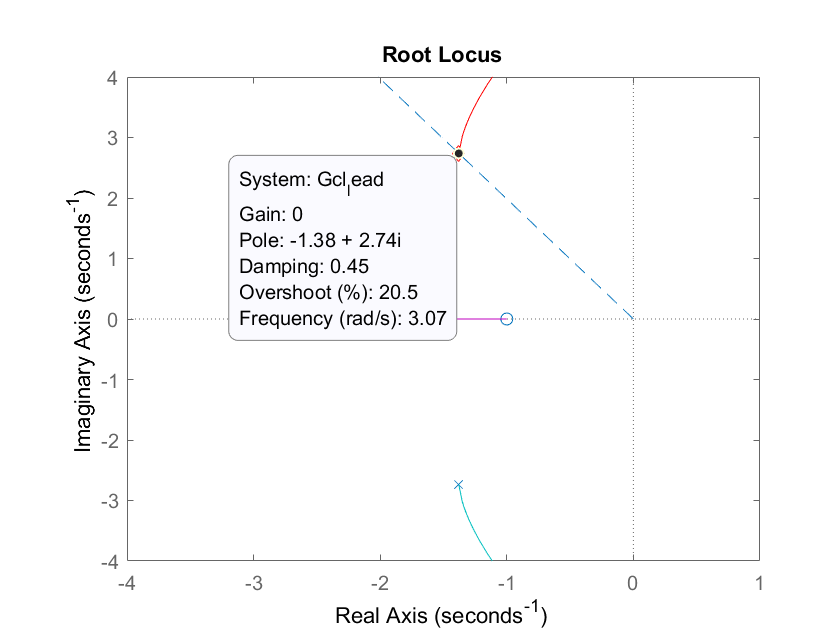
\includegraphics[width=0.48\linewidth]{../Q2_Lead_rlocus_a.png}}
	\subfigure[Step response.]{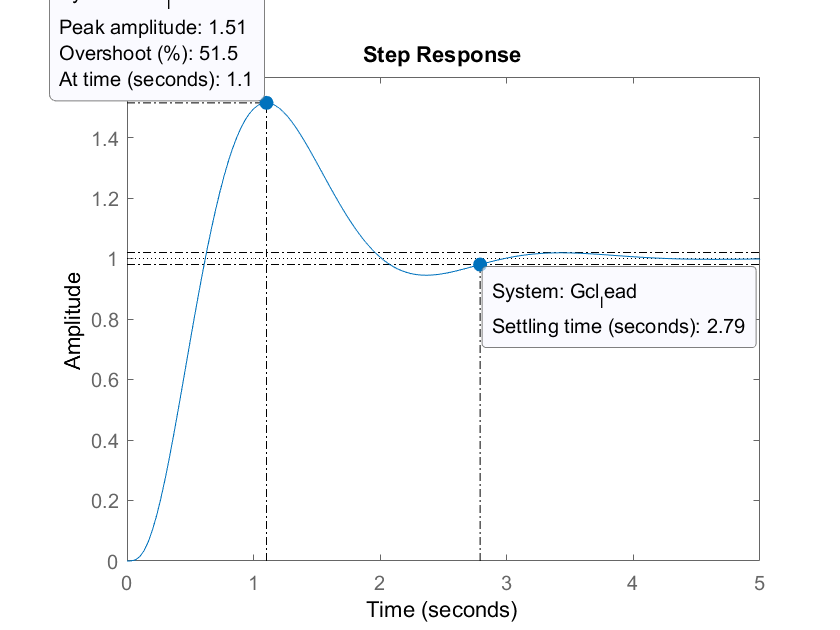
\includegraphics[width=0.48\linewidth]{../Q2_Lead_step_a.png}}
	\subfigure[Bode plot.]{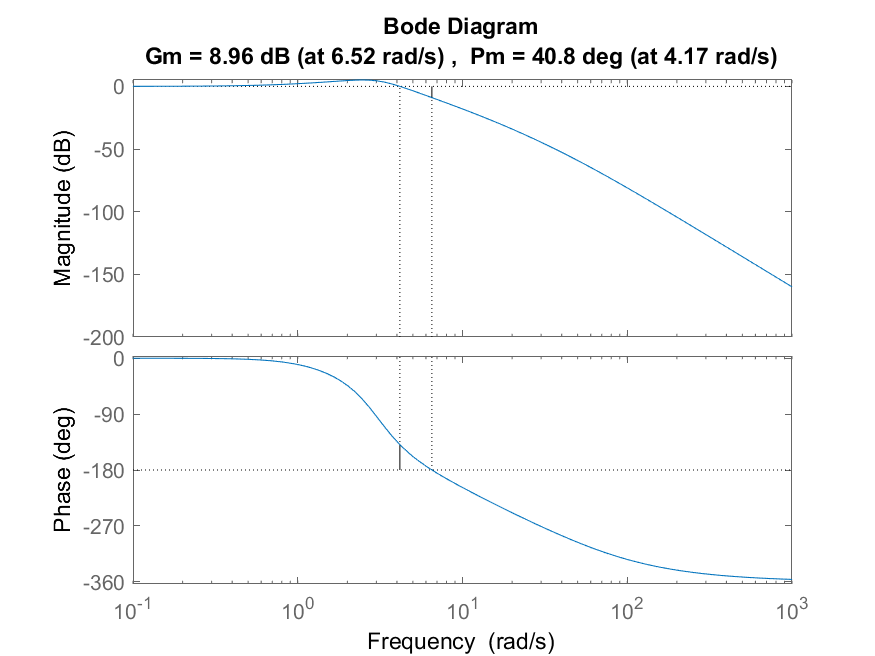
\includegraphics[width=0.48\linewidth]{../Q2_Lead_margin.png}}
	\caption{Closed-loop system with the Lead compensator.}
	\label{fig:Q2_lead}
\end{figure}

The script below simulates the Phase-Lead compensator.
\begin{lstlisting}[language=matlab, caption={}, label={}]
%% c) Phase lead compensator
z_lead = 1; % location of the desired zero
% using the angle condition to determine the location of the pole
x = -real(s1); y = imag(s1);
h = 180 + 180 - atand(y/(x-z_lead))-2*( 180-atand(y/x) )-atand(y/(a-x))...
-atand(y/(b-x));
p_lead = y/tand(h)+x;
% Gc compensator TF
Gc_lead = (s+z_lead)/(s+p_lead);
% obtaining the gain K with the gain condition equation
K = ((-x)^2+y^2)*sqrt((-x+a)^2+y^2)*sqrt((-x+b)^2+y^2)*...
sqrt((-x+p_lead)^2+y^2)/sqrt((-x+z_lead)^2+y^2);
% the open-loop system
G = K/(s^2*(s+a)*(s+b));% plant G
Gol_lead = Gc_lead*G; % open-loop with the Lead compensator
Gcl_lead = feedback(Gol_lead,1); % closed-loop with the Lead compensator

fig = figure(1);
rlocus(Gcl_lead);
hold;
% ploting the s1 and zeta in the rlocus
n = 0:1:160; m = n*sqrt(zeta^2/(1-zeta^2));
axis ([ -4 1 -4 4]);
plot (-m,n,'--'); % zeta
plot (-x,y,'rd');
saveas(fig,'Q2_Lead_rlocus.png');

fig = figure(2);
step(Gcl_lead);
saveas(fig,'Q2_Lead_step.png');

fig = figure(3);
margin(Gcl_lead);
saveas(fig,'Q2_Lead_margin.png');
BW_lead = bandwidth(Gcl_lead); % bandwidth
\end{lstlisting}


\subsection{Adding a Pre-filter}
The use of a Pre-filter in series with the closed-loop systems can reduce the overshoot canceling the effect of the Phase-Lead's zero.

The Pre-filter is written as follows,
\begin{align}
G_{pf} &= \dfrac{p}{s+p} \\
\intertext{where $p$ can be at the exact point of the $z_{lead}=1$,}
G_{pf} &= \dfrac{1}{s+1} \nonumber
\end{align} 
applying to the closed-loop Phase-Lead compensated system and evaluating it,
\begin{align}
G_{lead+prefilter} &= G_{pf}~ \dfrac{G_{ol}}{1+G_{ol}} \nonumber\\
G_{lead+prefilter} &=  \dfrac{1}{s+1} ~\dfrac{10047~(s+1)}{(s+50)(s+13.07)(s+1.64)(s^2+2.76~s+9.40)}\nonumber
\end{align}  

Fig. \ref{fig:Q2_lead+prefilter} shows the result of implementing a Pre-filter, where the overshoot decreases dramatically with a small change in the settling time.
\begin{figure}[H]
	\centering
	\subfigure[Step response.]{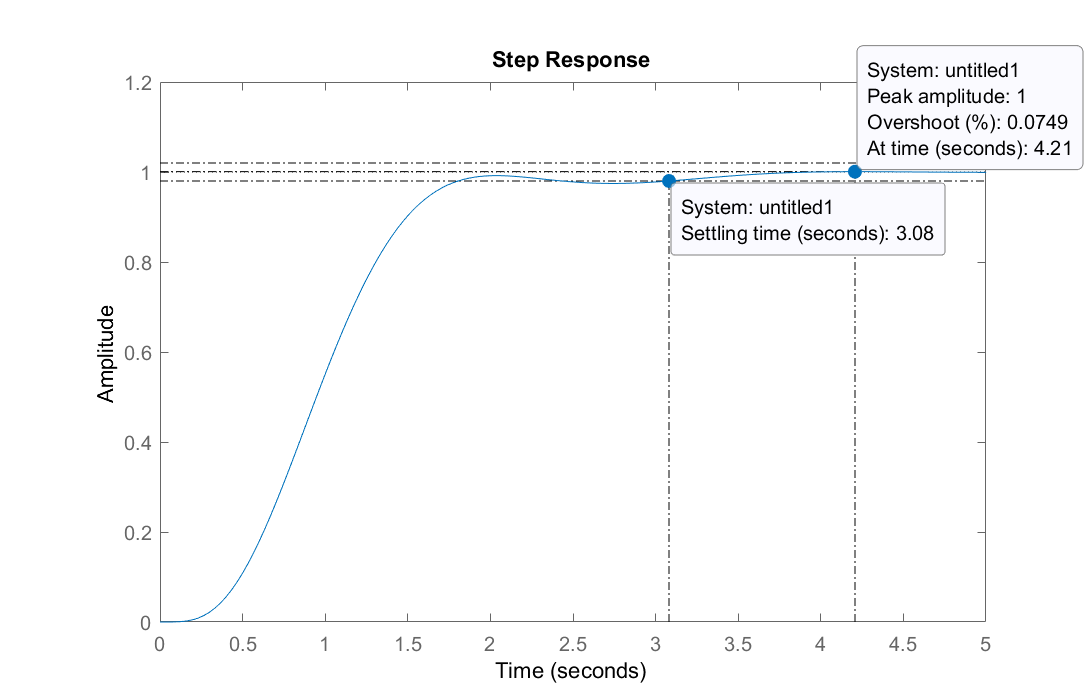
\includegraphics[width=0.52\linewidth]{../Q2_Lead+prefilter_step_a.png}}
	\subfigure[Bode plot]{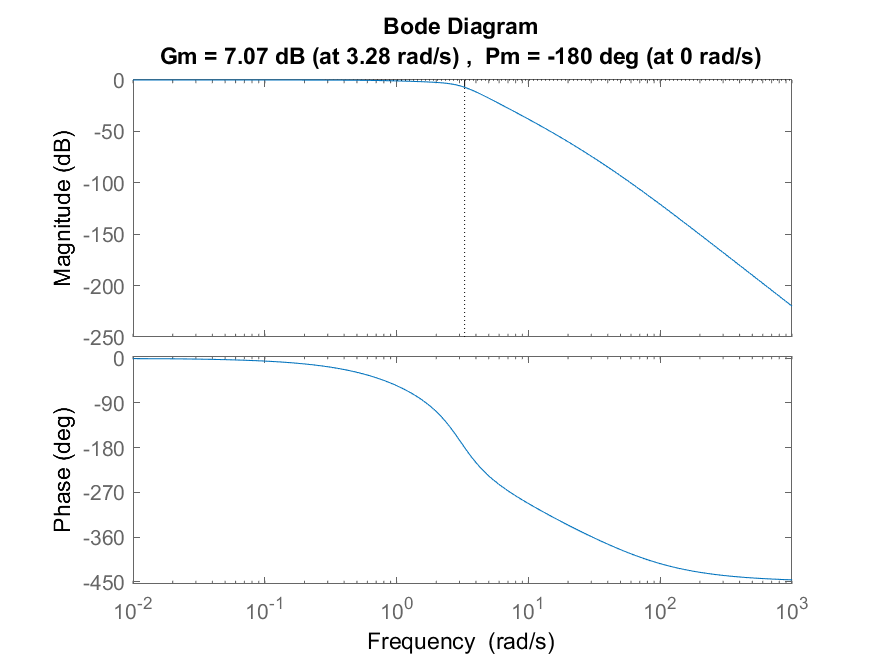
\includegraphics[width=0.44\linewidth]{../Q2_Lead+prefilter_margin.png}}
	\caption{Closed-loop Lead compensated in series with a Pre-filter.}
	\label{fig:Q2_lead+prefilter}
\end{figure}

The Matlab script below calculates and implements the Pre-filter.
\begin{lstlisting}[language=matlab, caption={}, label={}]
%% Using prefilter to reduce the overshoot
pf = z_lead; % selecting the zero of the lead compensator (z_lead)
Gpf = pf/(s+pf);

fig = figure(3);
step(Gpf*Gcl_lead);
saveas(fig,'Q2_Lead+prefilter_step.png');

fig = figure(4);
margin(Gpf*Gcl_lead);
saveas(fig,'Q2_Lead+prefilter_margin.png');
BW_lead_prefilter = bandwidth(Gpf*Gcl_lead); % bandwidth
\end{lstlisting}
  
\subsection{Design of the Phase-Lag compensator}
The Phase-Lag compensator has the following transfer function,
\begin{align}
G_{lag} = \dfrac{s+z_{lag}}{s+p_{lag}}, \quad |p_{lag}|< |z_{lag}|
\end{align}
This compensator will be used in series with the Phase-Lead compensator designed in the previous task. And now, the design requirement is the steady-state error ($ess_a$) for a parabolic input $0.5At^2\leq2.5\%$.

First, obtaining the LaPlace transform of the parabolic input,
\begin{align}
r(t) &= 0.5 A t^2, \quad R(s) = \frac{A}{s^3} \nonumber\\
\intertext{according to the final value theorem,}
ess &= \lim\limits_{s\rightarrow 0}~ s~\dfrac{A}{s^3} \dfrac{1}{1+G}  \\
\intertext{if $K_a = \lim\limits_{s\rightarrow 0} s^2~G$, the steady-state error is, } 
ess_a &= \dfrac{A}{K_a} \label{eq:ess_a}
\end{align}
where $K_a$ is the acceleration error constant.

If $ess_a=0.025$ and $A=1$, the \textbf{desired} acceleration error constant ($K_{a_d}$) is obtained using Eq.\eqref{eq:ess_a},
\begin{align}
K_{a_d} &= \frac{1}{ess_a} \nonumber\\
K_{a_d} &= 40 \nonumber\\
\intertext{and again, with $A=1$ and $G=G_{ol}$ from  Eq.\eqref{eq:Gol_lead}, the \textbf{actual} acceleration error constant $K_{a_{act}}$ is,}
K_{a_{act}} &= \lim\limits_{s\rightarrow 0} s^2~ G_{ol} = K_{a_{act}} = 2.67 \nonumber
\end{align}

The relation between the zero $z_{lag}$ and the pole $p_{lag}$ of the Phase-Lag compensator can be written as follows,
\begin{align}
\alpha &= \dfrac{K_{a_d}}{K_{a_{act}}} = \dfrac{z_{lag}}{p_{lag}}\\
\alpha &= 14.97 \nonumber\\
\intertext{choosing a $z_{lag}$ ten times smaller than the real part of the desired dominant pole $r_1$,}
z_{lag} &= \left| \dfrac{-1.38}{10} \right| \nonumber\\
z_{lag} &= 0.14 \nonumber\\
\intertext{and the pole should be,}
p_{lag} &= \dfrac{z_{lag}}{\alpha} \nonumber\\
p_{lag} &= 0.0092 \nonumber\\
\intertext{therefore, the Phase-Lag compensator becomes,}
G_{lag} &= \dfrac{s+0.14}{s+0.0092} \nonumber
\end{align}

The Matlab script of the Phase-Lag compensator is presented below.
\begin{lstlisting}[language=matlab, caption={}, label={}]
%% d) Phase-lag compensator
ess_a = 0.025; % steady-state error for a parabolic input 0.5At^2
Ka_d = 1/ess_a; % Ka desired
Ka_act = (z_lead/p_lead)*(K/(a*b));
% calculating the zero and pole of the compensator
alpha = Ka_d/Ka_act;
z_lag = abs(x)/10;
p_lag = z_lag/alpha;
% Gc phase-lag compensator
Gc_lag = (s+z_lag)/(s+p_lag);
\end{lstlisting}

\subsection{Evaluation of the performance}
Finally, the open-loop of the Phase-Lead compensator in series with the Phase-Lag compensator is written as follows,
\begin{align}
G_{ol1} &= G_{lag}~G_{lead} ~G(s) \label{eq:Gol_lead_lag}\\ 
G_{ol1} &= \dfrac{s+0.14}{s+0.0092}~ \dfrac{s+1}{s+8.36}~ \dfrac{10047}{s^2(s+9)(s+50)}  \nonumber\\
\intertext{and the Pre-filter with the closed-loop systems is,}
G_{lag+lead+prefilter} &= G_{pf}~ \dfrac{G_{ol1}}{1+G_{ol1}} \\
G_{lag+lead+prefilter} &= G_{pf}~ \dfrac{10047(s+1)(s+0.14)}{(s+50)(s+13.05)(s+1.78)(s+0.14)(s^2+2.51~s+8.75)} \nonumber
\end{align}

Fig. \ref{fig:Q2_all}c shows the step response of the system with and without the Pre-filter, it is clear that the Pre-filter reduces the overshoot in both cases with good settling time, the performance results can be seen in Table \ref{tab:Q2_all}. On the other hand, in Fig. \ref{fig:Q2_all}a, the desired dominant poles are slightly out of the root locus, it is recommended to add a second Phase-lead compensator in series in order correct that gap.
\begin{figure}[!ht]
	\centering
	\subfigure[Root locus of the Lead and Lag closed-loop compensator system.]{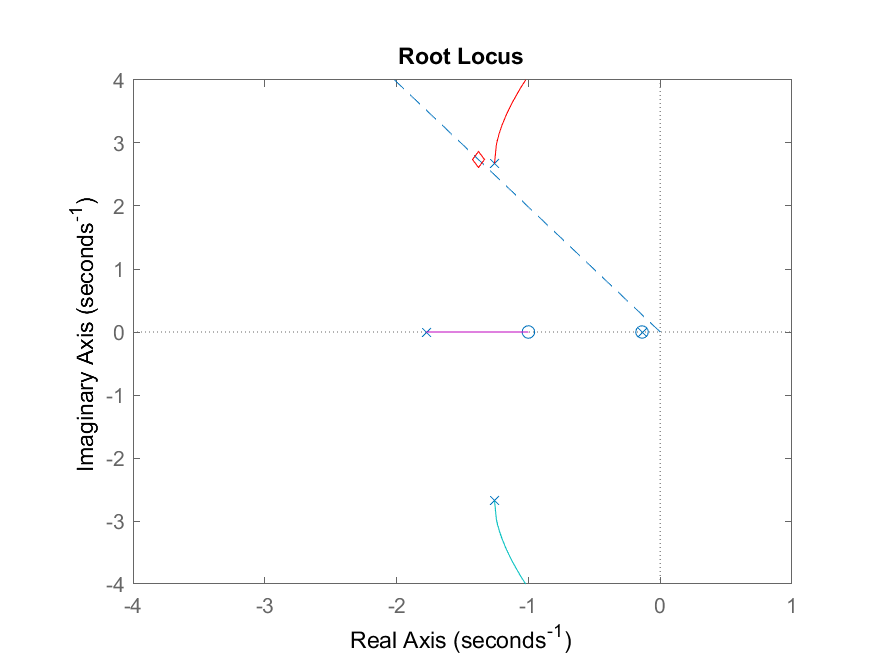
\includegraphics[width=0.48\linewidth]{../Q2_Lead+Lag_rlocus.png}}
	\subfigure[Bode plot of the closed-loop system.]{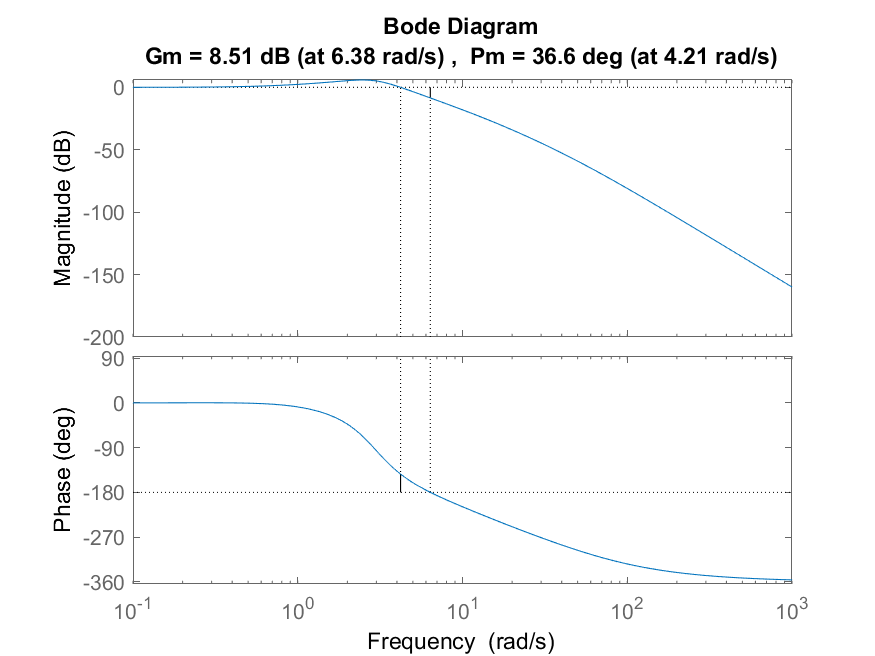
\includegraphics[width=0.48\linewidth]{../Q2_Lead+lag+prefilter_margin.png}}
	\subfigure[Step response of the closed-loop system.]{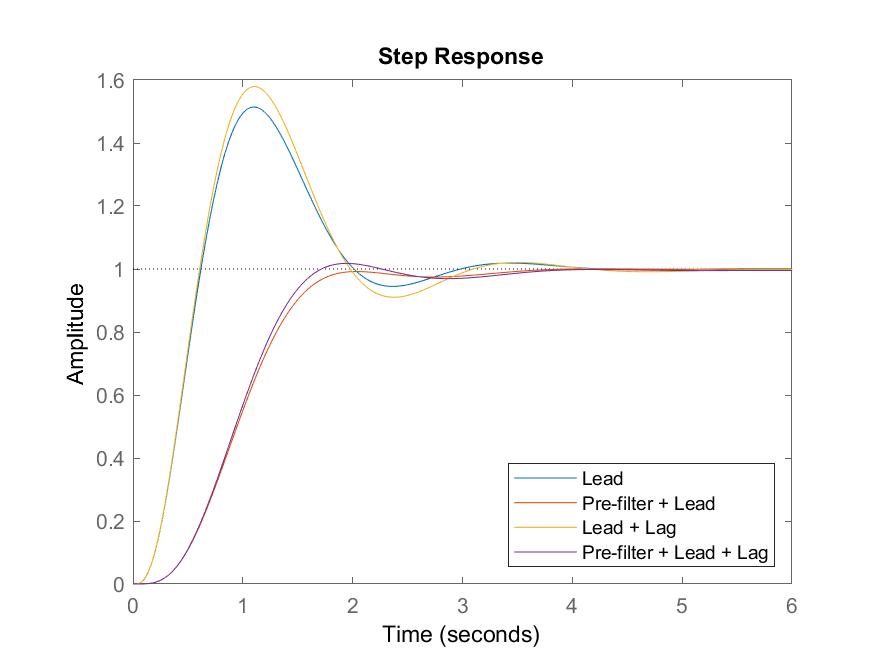
\includegraphics[width=0.7\linewidth]{../Q2_All_step_1.png}}
	\caption{Phase-lead, Phase-lag in series, and the Pre-filter.}
	\label{fig:Q2_all}
\end{figure}

\begin{table}[!ht]
	\centering
	\scalebox{1}{
		\begin{tabular}{p{3.7cm}|p{1cm}|p{2.8cm}|p{2cm}|p{3.5cm}}
			\bf{Quantity}        & \bf{Lead} & \bf{Prefilter+Lead} & \bf{Lead+Lag} & \bf{Prefilter+Lead+Lag} \\ \hline
			Rise Time            & 0.37      & 1.00                & 0.36          & 0.94                    \\ \hline
			Settling Time        & 2.79      & 3.08                & 3.59          & 3.31                    \\ \hline
			Percentage Overshoot & 51.46     & 0.07                & 57.96         & 1.79                    \\ \hline
			Phase Margin         & 40.80     & -180                & 36.60         & 36.60                   \\ \hline
			Gain Margin          & 8.96      & 7.07                & 8.51          & 8.51                    \\ \hline
			Bandwidth            & 4.87      & 2.31                & 4.89          & 2.58                    \\ \hline
			Peak Magnitude       & 1.51      & 1.00                & 1.58          & 1.02                    \\ \hline
		\end{tabular} 		
	}
	\caption{Performance evaluation to unit step response}
	\label{tab:Q2_all}
\end{table}

The following Matlab script was used to evaluate the performance of the previous systems.
\begin{lstlisting}[language=matlab, caption={}, label={}]
%% Evaluating the performance with the phase-lead, phase-lag and prefilter
Gol_lead_lag = Gc_lead*Gc_lag*G;
Gcl_lead_lag = feedback(Gol_lead_lag,1);

fig = figure(5); 
rlocus(Gcl_lead_lag);
hold;
% ploting the s1 and zeta in the rlocus
n = 0:1:160; m = n*sqrt(zeta^2/(1-zeta^2));
axis ([ -4 1 -4 4]);
plot (-m,n,'--'); % zeta
plot (-x,y,'rd');
saveas(fig,'Q2_Lead+Lag_rlocus.png');

fig = figure(6);
step(Gcl_lead,Gpf*Gcl_lead,Gcl_lead_lag,Gpf*Gcl_lead_lag)
legend('Lead','Pre-filter + Lead','Lead + Lag','Pre-filter + Lead + Lag'...
,'Location','southeast');
saveas(fig,'Q2_All_step_1.png');
stepinfo(Gpf*Gcl_lead_lag)

fig = figure(7);
margin(Gcl_lead_lag);
saveas(fig,'Q2_Lead+lag_margin.png');
BW_lead_lag = bandwidth(Gcl_lead_lag); % bandwidth

fig = figure(8);
margin(Gcl_lead_lag);
saveas(fig,'Q2_Lead+lag+prefilter_margin.png');
BW_lead_lag_prefilter = bandwidth(Gpf*Gcl_lead_lag); % bandwidth

%% Verifing Ka = 40
Ka = (z_lag/p_lag) * (z_lead/p_lead) * ( K/(a*b) );
ess_parabolic = a/Ka; 
\end{lstlisting}

\subsection{New Phase-Lead compensator}
Fig. \ref{fig:Q2_all}a demonstrates that the desired dominant closed-loop poles have moved slightly from the root locus, therefore, a new Phase-Lead compensator is calculated to correct that shift.

This time, the location of the zero is exactly below the real part of the desired pole, $z_{lead~2}=1.38$. Applying the angle condition with the desired pole $r_1$ as follows,

\begin{align}
&\measuredangle \left( \dfrac{s+z_{lead~2}}{s+p_{lead~2}} \quad \dfrac{s+z_{lag}}{s+p_{lag}} \quad \dfrac{s+z_{lead}}{s+p_{lead}} \quad \dfrac{K}{s^2(s+a)(s+b)}  \right) = -180\degree \\
&\measuredangle \left( \dfrac{r_1+z_{lead~2}}{r_1+p_{lead~2}} \quad \dfrac{r_1+z_{lag}}{r_1+p_{lag}} \quad \dfrac{r_1+z_{lead}}{r_1+p_{lead}} \quad \dfrac{K}{r_1^2(r_1+a)(r_1+b)}  \right) = -180\degree \nonumber \\
&\measuredangle z_{lead~2} +\measuredangle z_{lag} +\measuredangle z_{lead}   -  \measuredangle p_{lead~2} -\measuredangle p_{lag} - \measuredangle p_{lead} - 2~\measuredangle s -\measuredangle a - \measuredangle b = -180\degree \nonumber\\
\intertext{if, $r_1 = -x+j~y$ }
& \arctan\dfrac{y}{x-z_{lead~2}} + \left( 180\degree - \arctan\dfrac{y}{x-z_{lag}} \right) + \left( 180\degree-\arctan\dfrac{y}{x-z_{lead}} \right) ... \nonumber\\
& \quad - \arctan\dfrac{y}{p_{lead~2}} - \left( 180\degree-\arctan\dfrac{y}{x-p_{lag}}  \right)  -\arctan\dfrac{y}{p_{lead}-x} - 2\left( 180\degree -\arctan\dfrac{y}{x} \right) ... \nonumber\\
&\qquad -\arctan\dfrac{y}{a-x}-\arctan\dfrac{y}{b-x} = 180\degree \nonumber
\end{align}
after some operations,
\begin{align}
p_{lead~2} &= 1.48 \nonumber\\
\intertext{so, the second Phase-Lead compensator is,}
G_{lead~2} &= \dfrac{s+1.38}{s+1.48} \nonumber
\end{align}

Now, the new gain $K_{new}$ of the compensated system can be found using the gain condition,
\begin{align}
%&\left|  \dfrac{r_1+1}{r_1+8.38} \quad \dfrac{K}{r_1^2(r_1+9)(r_1+50)} \right| = 1 \nonumber\\
&\left| K_{new} \quad \dfrac{s+z_{lead~2}}{s+p_{lead~2}} \quad \dfrac{s+z_{lag}}{s+p_{lag}} \quad \dfrac{s+z_{lead}}{s+p_{lead}} \quad \dfrac{K}{s^2(s+a)(s+b)}  \right| = 1 \\
&\left| K_{new} \quad \dfrac{r_1+z_{lead~2}}{r_1+p_{lead~2}} \quad \dfrac{r_1+z_{lag}}{r_1+p_{lag}} \quad \dfrac{r_1+z_{lead}}{r_1+p_{lead}} \quad \dfrac{K}{r_1^2(r_1+a)(r_1+b)}  \right| = 1 \nonumber\\
&K_{new} = 1 \nonumber
\end{align}
which means that the gain has not changed.

The following script in Matlab simulates the previous results.
\begin{lstlisting}[language=tex, caption={}, label={}]
%% New phase-lead compensator
z_lead2 = x; % given zero lead right below the desired pole
f = 180 + atand(y/(x-z_lead2))+(180-atand(y/(x-z_lag)))...
+(180-atand(y/(x-z_lead))) - (180-atand(y/(x-p_lag)))-atand(y/(p_lead-x))...
-2*(180-atand(y/x))-atand(y/(a-x))-atand(y/(b-x));
% p_lead2 = y/tand(180+f) - x;
p_lead2 = y/tand(f) + x;
Gc_lead2 = (s+z_lead2)/(s+p_lead2);
% Calculating the new gain K with the lead 2 compensator
K_new = sqrt((-x+p_lead2)^2+y^2)*sqrt((-x+p_lag)^2+y^2)*...
sqrt((-x+p_lead)^2+y^2)*((-x)^2+y^2)*sqrt((-x+a)^2+y^2)*sqrt((-x+b)^2+y^2)/...
( sqrt((-x+z_lead)^2+y^2)*sqrt((-x+z_lag)^2+y^2)*sqrt((-x+z_lead)^2+y^2)*K );
Gol_lead2_lead_lag = K_new*Gc_lead2*Gol_lead_lag;
Gcl_lead2_lead_lag = feedback(Gol_lead2_lead_lag,1);
%% Verifing Ka = 40 
Ka_new = K_new*(z_lead2/p_lead2)*(z_lag/p_lag)*(z_lead/p_lead)*(K/(a*b));
ess_parabolic_new = a/Ka_new; 
\end{lstlisting}


\subsection{Evaluation of the performance with the second Phase-Lead compensator}
The open-loop of the new Phase-Lead compensator in series with the previous compensators is written as follows,
\begin{align}
G_{ol2} &= G_{lead~2}~G_{lag}~G_{lead} ~G(s) \label{eq:Gol_lead_lag_lead2}\\ 
G_{ol2} &= \dfrac{s+1.38}{s+1.48}\quad \dfrac{s+0.14}{s+0.0092} \quad \dfrac{s+1}{s+8.36} \quad \dfrac{10047}{s^2(s+9)(s+50)}  \nonumber\\
\intertext{and the Pre-filter with the closed-loop systems is,}
G_{lag+lead+prefilter} &= G_{pf}~ \dfrac{G_{ol2}}{1+G_{ol2}} \\
G_{lag+lead+prefilter} &= G_{pf}~ \dfrac{10047(s+1.38)(s+1)(s+0.14)}{(s+8.36)(s+1.48)(s+0.009)s^2(s+9)(s+50)} \nonumber
\end{align}

From Fig. \ref{fig:Q2_all_2}a it can be seen that the desired closed-loop poles are exactly in the root locus. Also, the $PM$ has changed a little with respect of the previous compensated system, from $36.60\degree$ to $39.50\degree$, Fig. \ref{fig:Q2_all_2}b. On the other hand, the step response has been improved with the Pre-filter and the new Phase-Lead compensator, see Table \ref{tab:Q2_all_2}.

\begin{figure}[!ht]
	\centering
	\subfigure[Root locus]{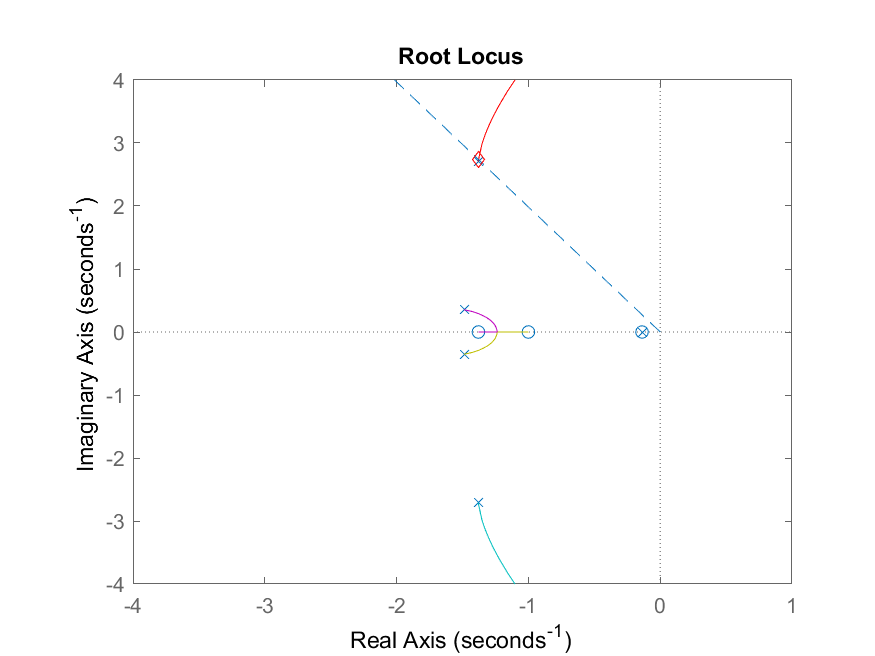
\includegraphics[width=0.48\linewidth]{../Q2_Lead2+Lead+Lag_rlocus.png}}
	\subfigure[Bode plot of the open-loop system without the  Pre-filter.]{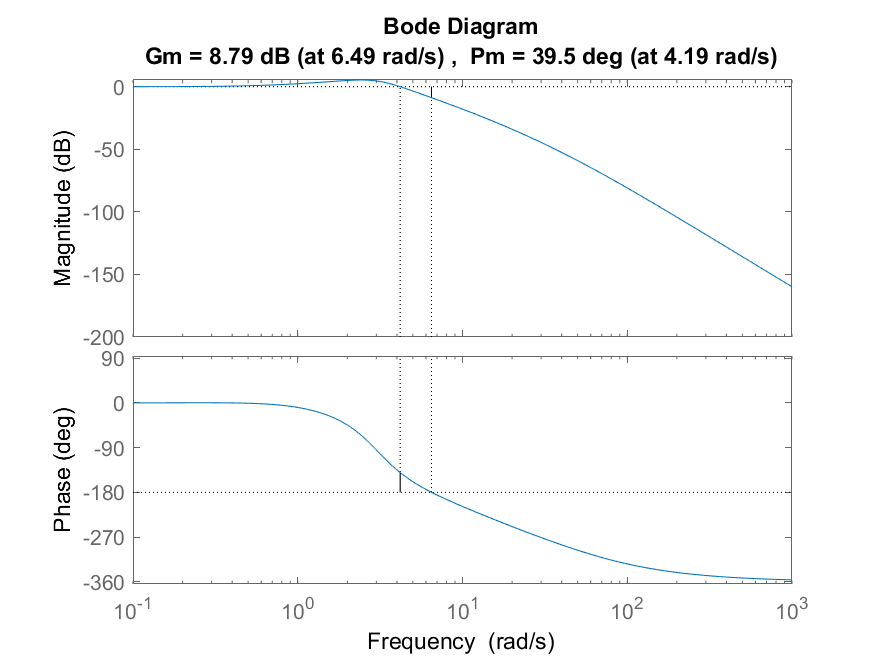
\includegraphics[width=0.48\linewidth]{../Q2_Lead2+lead+lag_margin.png}}
	\subfigure[Bode plot of the closed-loop system with the Pre-filter]{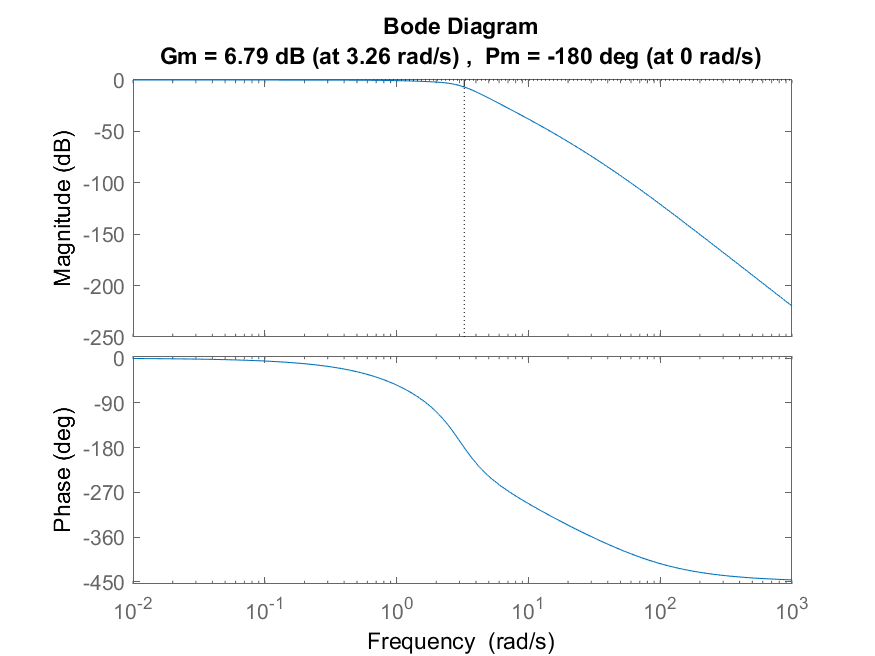
\includegraphics[width=0.48\linewidth]{../Q2_Lead2+lead+lag+prefilter_margin.png}}
	\subfigure[Step response of the closed-loop system.]{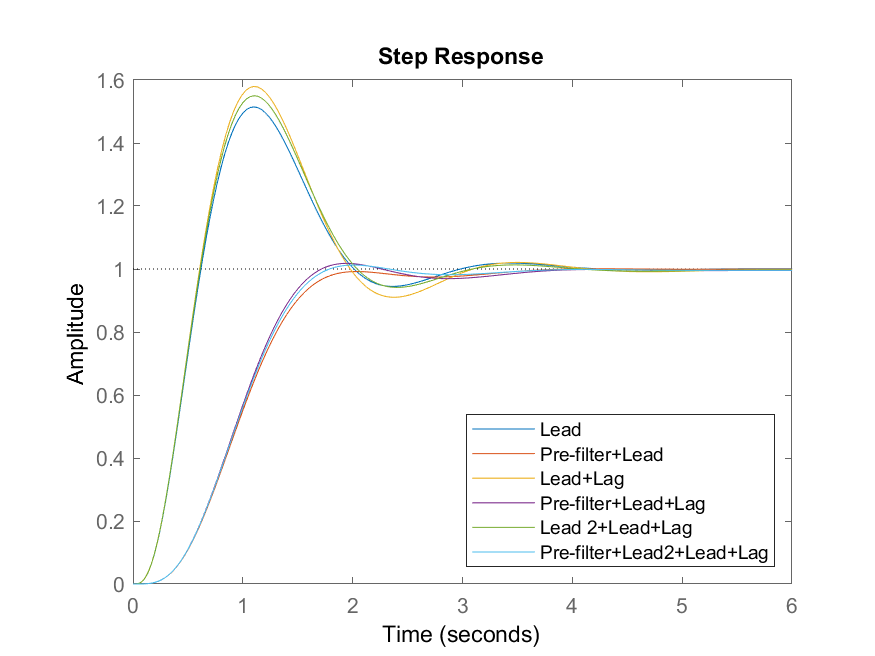
\includegraphics[width=0.48\linewidth]{../Q2_All_step_2.png}}
	\caption{Phase-lead 2, Phase-lead, Phase-lag in series, and the Pre-filter.}
	\label{fig:Q2_all_2}
\end{figure}

\begin{table}[!ht]
	\centering
	\scalebox{1}{
		\begin{tabular}{p{2.8cm}|p{1cm}|p{1.5cm}|p{1.5cm}|p{2cm}|p{2cm}|p{2cm}}
			\bf{Quantity}        & \bf{Lead} & \bf{Prefilter +Lead} & \bf{Lead +Lag} & \bf{Prefilter +Lead +Lag} & \bf{Lead\_2 +Lead +Lag} & \bf{Prefilter +Lead\_2 +Lead +Lag} \\ \hline
			Rise Time            & 0.37      & 1.00                & 0.36          & 0.94                    & 0.37                 & 0.97                           \\ \hline
			Settling Time        & 2.79      & 3.08                & 3.59          & 3.31                    & 2.87                 & 1.68                           \\ \hline
			Percentage Overshoot & 51.46     & 0.07                & 57.96         & 1.79                    & 55.00                & 1.25                           \\ \hline
			Phase Margin         & 40.80     & -180                & 36.60         & 36.60                   & 39.50                & -180                           \\ \hline
			Gain Margin          & 8.96      & 7.07                & 8.51          & 8.51                    & 8.79                 & 6.79                           \\ \hline
			Bandwidth            & 4.87      & 2.31                & 4.89          & 2.58                    & 4.88                 & 2.42                           \\ \hline
			Peak Magnitude       & 1.51      & 1.00                & 1.58          & 1.02                    & 1.55                 & 1.01                           \\ \hline
		\end{tabular} 		
	}
	\caption{Performance evaluation to unit step response}
	\label{tab:Q2_all_2}
\end{table}
The following script in Matlab simulates the previous results.
\begin{lstlisting}[language=tex, caption={}, label={}]
%% Comparing the new compensator of the previous designs.
fig = figure(9);
rlocus(Gcl_lead2_lead_lag)
hold on;
% ploting the s1 and zeta in the rlocus
n = 0:1:160; m = n*sqrt(zeta^2/(1-zeta^2));
axis ([ -4 1 -4 4]);
plot (-m,n,'--'); % zeta
plot (-x,y,'rd');
saveas(fig,'Q2_Lead2+Lead+Lag_rlocus.png');

fig = figure(10);
% step(Gcl_lead2_lead_lag,Gpf*Gcl_lead2_lead_lag)
step(Gcl_lead,Gpf*Gcl_lead,Gcl_lead_lag,Gpf*Gcl_lead_lag,...
Gcl_lead2_lead_lag,Gpf*Gcl_lead2_lead_lag)
legend('Lead','Pre-filter+Lead','Lead+Lag','Pre-filter+Lead+Lag'...
,'Lead 2+Lead+Lag','Pre-filter+Lead2+Lead+Lag','Location','southeast');
saveas(fig,'Q2_All_step_2.png');
stepinfo(Gpf*Gcl_lead2_lead_lag)

fig = figure(11);
margin(Gcl_lead2_lead_lag);
saveas(fig,'Q2_Lead2+lead+lag_margin.png');
BW_lead2_lead_lag = bandwidth(Gcl_lead2_lead_lag); % bandwidth

fig = figure(12);
margin(Gpf*Gcl_lead2_lead_lag);
saveas(fig,'Q2_Lead2+lead+lag+prefilter_margin.png');
BW_lead2_lead_lag_prefilter = bandwidth(Gpf*Gcl_lead2_lead_lag); % bandwidth
\end{lstlisting}


\subsection{Conclusion}
The settling time requirement $t_s\leq2.9$ was satisfied by three of the six compensators, and only the last one with the Pre-filter achieved the desired overshoot $P.O.\leq 20 \%$. It is clear that the use of the Pre-filter reduces the overshoot drastically.  








\printbibliography
\end{document}
